% Filename  : samplepaper.tex
% Purpose   : A sample exam paper to demonstrate how to use the 'ditpaper'
%             TeX class.
% Author    : Emmet Caulfield
% Revision  : $Id: samplepaper.tex 2 2006-02-19 20:34:45Z emmet $
% Repository: $HeadURL: http://svn.netrogen.lan/tex-ditpaper/trunk/samplepaper.tex $
%

% 'nosolution' (default) and 'solution' toggle the inclusion of solutions
% in the output. The tag --SOLUTION-OPTION--, below, is replaced by 'sed' 
% in the Makefile to cause both the paper and the solutions to be produced.
\documentclass[--SOLUTION-OPTION--]{ditpaper}

\usepackage{graphicx}
\usepackage{multirow}

% These must be set or bizarre defaults will be used:
\facility{Kevin Street, Dublin 8}
\course{BSc (Hons) in Computer Science}
\examcode{R228/406}
\stage{Stage 4}
\session{Supplemental Examinations 2008}
\title{Artificial Intelligence 2}
\examiners{Dr. John Kelleher\\
Prof. B. O'Shea\\
Dr. I. Arana}
\examdate{}
\examtime{Duration: 2 Hours}
\instructions{Answer Question 1 (40 marks) \textbf{and}\par{} any 2 Other Questions (30 marks each).}

\begin{document}

% questions from across the course
\question
\begin{enumerate}

	\item The logical operator $\iff$ is read \emph{if and only if}. $P \iff Q$ is defined as being equivalent to $(P \Rightarrow Q) \land (Q \Rightarrow P)$.  Based on this definition, show using truth tables the logical equivalence of $P \iff Q$ and $P \lor Q \Rightarrow P \land Q$.
		\marks{5}
		\begin{answer}
			\begin{tabular}{|c|c|c|c|c|c|}
				P & Q & $(P \Rightarrow Q) \land (Q \Rightarrow P)$ & $P \lor Q$ & $P \land Q$ & $(P \lor Q) \Rightarrow ( P \land Q)$\\ 
				\hline
				T & T & T & T & T & T \\
				T & F & F & T & F & F \\
				F & T & F & T & F & F \\
				F & F & T & F & F & T \\
			\end{tabular}
		\end{answer}

	\item Distinguish between \textbf{false negatives} and \textbf{false positives}.
		\marks{5}
		\begin{answer}
			\begin{description}
				\item [False negative] an example can be a false negative for the hypothesis, if the hypothesis says it should be negative but in fact it is positive.
				\item [False positive] an example can be a false positive for the hypothesis, if the hypothesis says it should be positive but in fact it is negative.
			\end{description}
		\end{answer}

	\item In the context of machine learning, explain what is meant by \textbf{overfitting} the training data.	
		\marks{5}
		\begin{answer}
			Overfitting occurs when classifiers make decisions based on accidental properties of the training set that will lead to errors on the test set (or new data). As a result, whenever there is a large set of possible hypotheses, one has to be careful not to use the resulting freedom to find meaningless "regularity" in the data.
		\end{answer}

	\item In the context of inductive learning explain what is meant by a \textbf{consistent hypothesis}.
		\marks{5}
		\begin{answer}
			A hypothesis is consistent if it agrees with the true function on all examples that we have.
		\end{answer}
		
	\item Describe the problems associated with measuring \textbf{classifier performance} using a single accuracy figure. Describe a more appropriate alternative.
	\marks{20}
	\begin{answer}
		This is a discursive question so giving a precise answer is not appropriate. However, an answer to this question should describe how a single accuracy figure can hide a classifier's real performance. An example should be provided such as the following:
		
		\begin{itemize}
			\item Text cases: 1000
			\item Positive examples: 900
			\item Negative examples: 100
		\end{itemize}
		
		Assuming the classifier always classifies positively then its accuracy on the given text set would be 90\% which is not an accurate reflection of the classifiers performance.
		
		 The most obvious alternative would be to describe the use of \textbf{specificity}, \textbf{sensitivity} and \textbf{precision} along with a \textbf{confusion matrix}. Students should explain how a confusion matrix can be use as follows:
		 
				\begin{tabular}{|c|c|c|c|}
				\multicolumn{2}{|c|}{Classifier Results} & & \\
				Class A (yes) & Class B (no) &  & \\
				\hline
				Correct & $F_{n}$ & Class A (yes) & \multirow{2}{*}{Expected Results}\\
				$F_{p}$ & Correct & Class B (no) & \\
				\end{tabular}
		
		And finally it is expected that the students would describe specificity, sensitivity and precision as follows:
		
		$sensitivity = \frac{t_{pos}}{pos}$
		$specificity = \frac{t_{neg}}{neg}$
		$precision = \frac{t_{pos}}{t_{pos}+f_{pos}}$
		
	\end{answer}

		
\end{enumerate}



%Q2 30 marks
% reasoning under uncertainty
% aima chapters 13, 14, 15
\question
\begin{enumerate}
	\item Consider the domain of dealing 5-card poker hands from a standard deck of 52 cards, under the assumption that the dealer is fair.
		\begin{enumerate}
			\item Given that the number of combinations of $r$ objects that can be selected,  without regard to order and without repetition, from $n$ distinct objects is given by the equation ${n \choose r} = \frac{n!}{(n-r)!r!}$, how many atomic events are there in the joint probability distribution (i.e., how many 5-card hands are there)?
				\marks{5}
				\begin{answer}
					There are ${52 \choose 5} = \frac{52!}{(47! 5!} = \frac{52 \times 51 \times 50 \times 49 \times 48}{1 \times 2 \times 3 \times 4 \times 5} = 2,598,960$ possible five-card hands
				\end{answer}
			\item What is the probability of each atomic event?
				\marks{5}
				\begin{answer}
					By the fair-dealing assumption, each of these is equally likely. Each hand therefore occurs with probability 1/2,598,960. 
				\end{answer}
			\item What is the probability of being dealt a royal flush (i.e. being dealt a hand containing Ace, King, Queen, Jack and 10 all from the one suit)?
				\marks{5}
				\begin{answer}
					There are four hands that are royal straight flushes (one in each suit). These events are are mutually exclusive, therefore the probability of a royal �ush is just the sum of the probabilities of the atomic events, i.e., $\frac{4}{2,598,960} = \frac{1}{649,740}$. 
				\end{answer}
			\item What is the probability of being dealt a four of a kind (i.e. four kings, or four nines etc.)?
				\marks{5}
				\begin{answer}
					There are 13 possible �kinds� and for each, the �fth card can be one of 48 possible other cards. The total probability is therefore $\frac{13 \times 48}{2, 598, 960} = \frac{1}{4,165}$. 
				\end{answer}
		\end{enumerate}
	\item Consider the Bayesian network for car diagnosis shown in Figure \ref{fig:carsystem}.
		\begin{enumerate}
			\item Extend the network with the Boolean variables \textit{IcyWeather} and \textit{StarterMotor}. \textit{Note, cold weather normally affects the battery and start motor of a car}. 
				\marks{5}
				\begin{answer}
					\textit{Icy Weather} is not caused by any of the car-related variables, so needs no parents. It directly affects the battery and the starter motor. \textit{StarterMotor} is an additional precondition for Starts.
					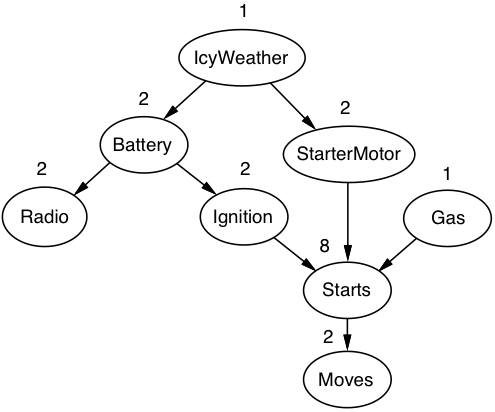
\includegraphics[width=2.5in]{./images/car-extended.png}
				\end{answer}
			\item How many independent values are contained in the joint probability?
				\marks{5}
				\begin{answer}
					With 8 Boolean variables, the joint has $2^{8}-1 = 255$ independent entries. 
				\end{answer}
		\end{enumerate}
\end{enumerate}
\begin{figure}
	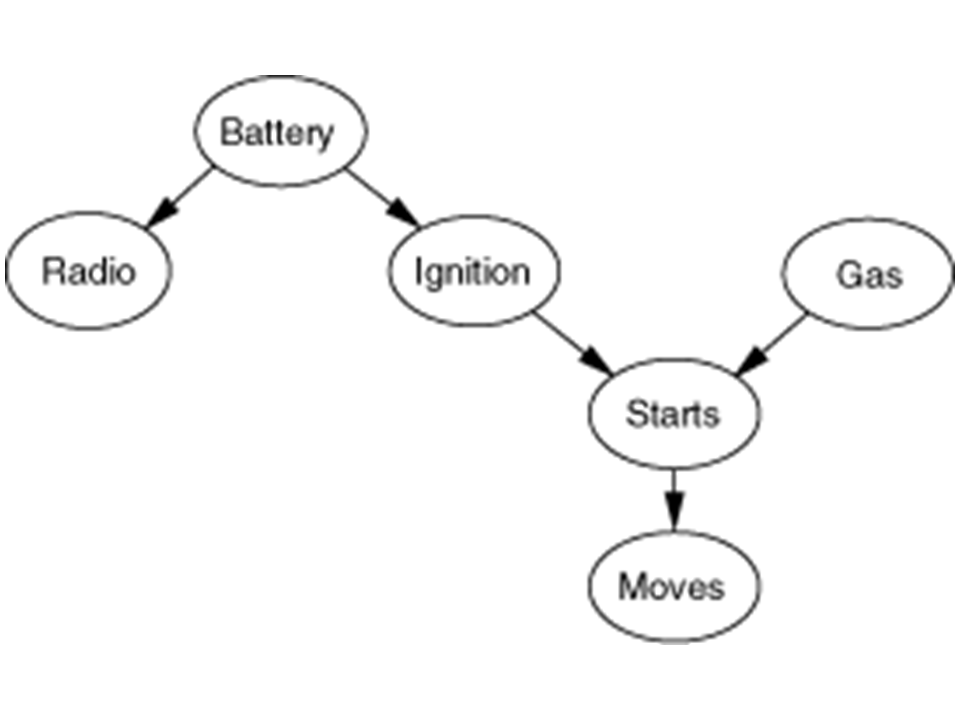
\includegraphics[width=2.5in]{./images/car-starts.png}
	\caption{A Bayesian network of a car's electrical system and engine. Each variable is boolean and the true value indicates that the corresponding aspect of the vehicle is in working order.}
	\label{fig:carsystem}
\end{figure}

\newpage

%Q3
%Inductive Learning (Decision Trees)
%aima chapters 18
\question
\begin{enumerate}

	\item Suppose we generate a training set from a decision tree and then apply decision-tree learning to the training set. Is it the case that the learning algorithm will eventually return the correct tree as the training set size goes to infinity? Why or why not?
		\marks{5}
		\begin{answer}
				The algorithm may not return the''correct'' tree, but it will return a tree that is logically equivalent, assuming that the method for generating examples eventually generates all possible combinations of input attributes. This is true because any two decision tree defined on the same set of attributes that agree on all possible examples are, by de�nition, logically equivalent. The actual form of the tree may differ because there are many different ways to represent the same function. (For example, with two attributes A and B we can have one tree with $A$ at the root and another with $B$ at the root.) The root attribute of the original tree may not in fact be the one that will be chosen by the information gain heuristic when applied to the training examples. 
		\end{answer}

	\item In the context of inductive logic learning, what is meant by the \textbf{extension} of a hypothesis?
		\marks{5}
		\begin{answer}
			Each hypothesis predicts that a certain set of examples, namely those that satisfy the hypotheses definition, are examples that satisfy the goal predicate. This set of examples is called the extension of the hypothesis. For example, assuming a standard interpretation, the extension of the predicate $digit(X)$ is $\{1,2,3,4,5,6,7,8,9,0\}$
		\end{answer}

	\item Distinguish between the \textbf{generalisation} and \textbf{specialization} of a logical predicate.
		\marks{10}
		\begin{answer}
			The generalisation of a logical predicate results in the broadening of the extension of the predicate. Some of the operations that can be used to generalise a logical predicate include: converting conjunctions in the predicate to disjunctions or dropping conditions in the predicate. You would generalise a predicate in response to recognising a false negative.
The specialisation of a logical predicate results in the narrowing of the extension of the predicate. Some of the operations that can be used to generalise a logical predicate include: converting disjunctions in the predicate to conjunctions or adding conditions in the predicate. You would specialise a predicate in response to recognising a false positive.
 		\end{answer}
	
	\item For some data sets it is possible to devise multiple hypotheses that are consistent with the data. Describe a heuristic for choosing among multiple consistent hypotheses and explain why your heuristic is reasonable.
		\marks{10}
		\begin{answer}
			One answer is to use Occam�s razor (sometimes called Ockham�s razor) : prefer the hypothesis that maximizes a combination of simplicity and consistency with the data. This makes sense, because hypotheses that are no simpler than the data themselves are failing to extract any pattern from the data. Defining simplicity is not easy but it seems reasonable to say that a degree-1 polynomial is simpler than a degree-12 polynomial.
		\end{answer}

\end{enumerate}
 
%Q4
%Neural Nets
\question 
\begin{enumerate}
	\item What does it mean if two classes $C_1$ and $C_2$ are described as \textbf{linearly separable}.
		\marks{5}
		\begin{answer}
			This means that for each class $C_i$ there exists a hyperplane $H_i$ such that on its positive side lie all $x \in C_i$ and on its negative side lie all $x \in C_j , j \ne i$
		\end{answer}
 
	\item Describe the processing stages of a McCulloch-Pits ''unit''.
		\marks{10}
		\begin{answer}
			The processing stages of a unit are:
			\begin{enumerate}
				\item Each unit $i$ first compute a weighted sum of its inputs:  $in_i \leftarrow \sum_j W_{j,i}  a_j$
				\item Then it applies an \textbf{activation function} $g$ to this sum to derive the output (activation) $a_i$: $a_i \leftarrow g(in_i) = g\left(\sum_j W_{j,i} a_j\right)$
			\end{enumerate}

			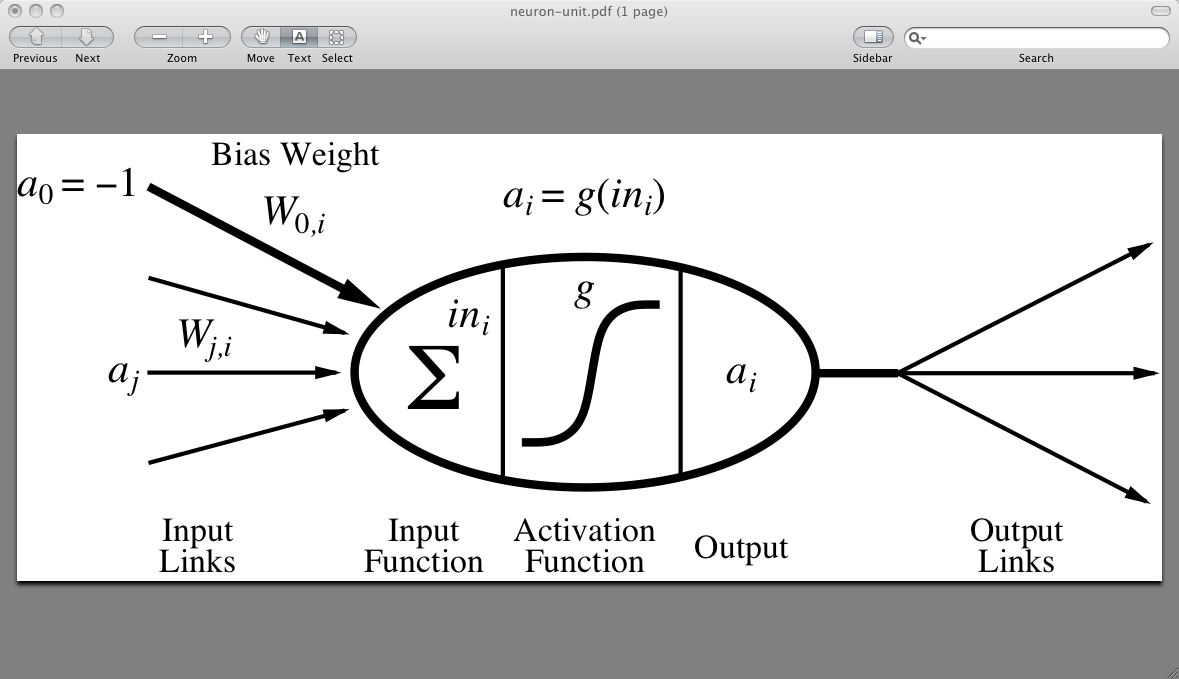
\includegraphics[width=3.5in]{./images/neuron-unit.png}
		\end{answer}

 
	\item Construct by hand a neural network that computes the XOR function of two inputs. Make sure to specify what sort of units you are using.
		\marks{15}
			\begin{answer}
				XOR (in fact any Boolean function) is easiest to construct using step-function units. Because XOR is not linearly separable, we will need a hidden layer. It turns out that just one hidden node suf�ces. To design the network, we can think of the XOR function as OR with the AND case (both inputs on) ruled out. Thus the hidden layer computes AND, while the output layer computes OR but weights the output of the hidden node negatively. The image below illustrates the network.
			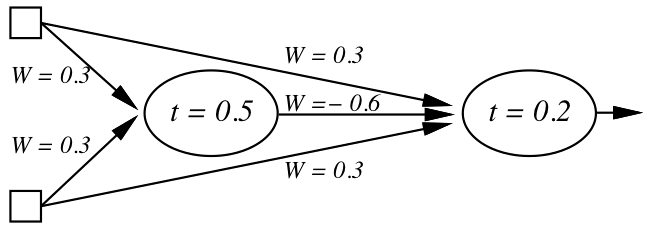
\includegraphics[width=3.5in]{./images/xor-mlp.png}
		\end{answer}
\end{enumerate}


\end{document}
